\documentclass{beamer}
\usetheme[numbering = fraction, progressbar = frametitle]{metropolis}           % Use metropolis theme
\usepackage{pgf,tikz,pgfplots}
\pgfplotsset{compat=1.15}
\usepackage{mathrsfs}
\usetikzlibrary{arrows}
\pagestyle{empty}

\usepackage{animate}
\usepackage[font=small,labelfont=bf]{caption}
\usepackage{tikz}
\usetikzlibrary{positioning}

\usepackage{algorithm}
\usepackage{algorithmic}


\usepackage[backend=bibtex]{biblatex}
\usepackage{filecontents}
\begin{filecontents}{\jobname.bib}
  @article{DBLP:journals/corr/KollaJG16,
    author    = {Ravi Kumar Kolla and
                 Krishna P. Jagannathan and
                 Aditya Gopalan},
    title     = {Stochastic bandits on a social network: Collaborative learning with
                 local information sharing},
    journal   = {CoRR},
    volume    = {abs/1602.08886},
    year      = {2016},
    url       = {http://arxiv.org/abs/1602.08886},
    archivePrefix = {arXiv},
    eprint    = {1602.08886},
    timestamp = {Mon, 13 Aug 2018 16:47:14 +0200},
    biburl    = {https://dblp.org/rec/bib/journals/corr/KollaJG16},
    bibsource = {dblp computer science bibliography, https://dblp.org}
  }
\end{filecontents}

\addbibresource{\jobname.bib}

\setbeamercolor{normal text}{bg=white}

\usepackage{stmaryrd}

\addtobeamertemplate{navigation symbols}{}{%
    \usebeamerfont{footline}%
    \usebeamercolor[fg]{footline}%
    \hspace{1em}%
    \insertframenumber/\inserttotalframenumber
}

\title{Bandit networks}
\date{January 24, 2019}
\author{Charles \textsc{Auguste} \& Louis \textsc{Trezzini}}
%\institute{Centre for Modern Beamer Themes}
\setbeamercolor{normal text}{bg=white}

\begin{document}

\maketitle

\begin{frame}{Goals of the project}
Review the article \fullcite{DBLP:journals/corr/KollaJG16}

\begin{itemize}
  \item Understand the proposed framework and algorithms
  \item Implement them and reproduce the experimental results
  \item Pinpoint the limitations of the model and try to improve it
\end{itemize}
\end{frame}

\begin{frame}{Multi-agent stochastic multi-armed bandit (MAB) problem}
\begin{itemize}
  \item Undirected graph $G = (V, E)$ with $|V| = m$ users
  \item All users are playing the \alert{same} MAB problem with $K$ arms
  \item A user $v$ can observe the actions and the respective rewards of itself and its one hop neighbors up to round $t$, before deciding the action for round $(t+1)$
  \item $\mathcal{N}(v)$: node $v$ and its one-hop neighbors
  \item $m^v_i(t)$: number of times arm $i$ has been chosen by node $v$ and its one-hop neighbors up to round $t$
  \item $\hat{\mu}_{m_i^v(t)}$: average reward for playing arm $i$ obtained by node $v$ and its one-hop neighbors up to round $t$
\end{itemize}

\end{frame}

\begin{frame}{Upper-Confidence-Bound-Network (UCB-Network) policy}
  \begin{algorithmic}
     \STATE {Each user in $G$ follows UCB-user policy}
     \STATE{\bfseries UCB-user policy for a user $v$:}
     \STATE{~~\bfseries Initialization:} For $1 \leq t \leq K$
     \STATE{~~~~- play arm $t$}
     \STATE{~~\bfseries Loop:} For $K \leq t \leq n$
     \STATE{~~~~ - $a^v(t+1) = \underset{j}{\operatorname{argmax}} \, \, \hat{\mu}_{m_j^v(t)} + \sqrt{\frac{2 \ln t}{m_j^v(t)}}$}
  \end{algorithmic}
\end{frame}

\begin{frame}{Follow Your Leader (FYL) policy}
  \begin{algorithmic}
    \STATE {\bfseries Input:} Graph $G$, a dominating set $D$ and a dominating set partition
    \STATE{\bfseries Leader - Each node in $D$:}
    \STATE{Follows the UCB-user policy by using the samples of itself and its neighbors}
    \STATE{\bfseries Follower - Each node in $V\setminus D$:}
    \STATE{In round $t=1$:}
    \STATE{~~~~- Chooses an action randomly from $\mathcal{K}$}
    \STATE{In round $t > 1$:}
    \STATE{~~~~-  Chooses the action taken by the leader in its component, in the previous round $(t-1)$}
 \end{algorithmic}
\end{frame}


\begin{frame}{Issue with the FYL policy}
\begin{figure}
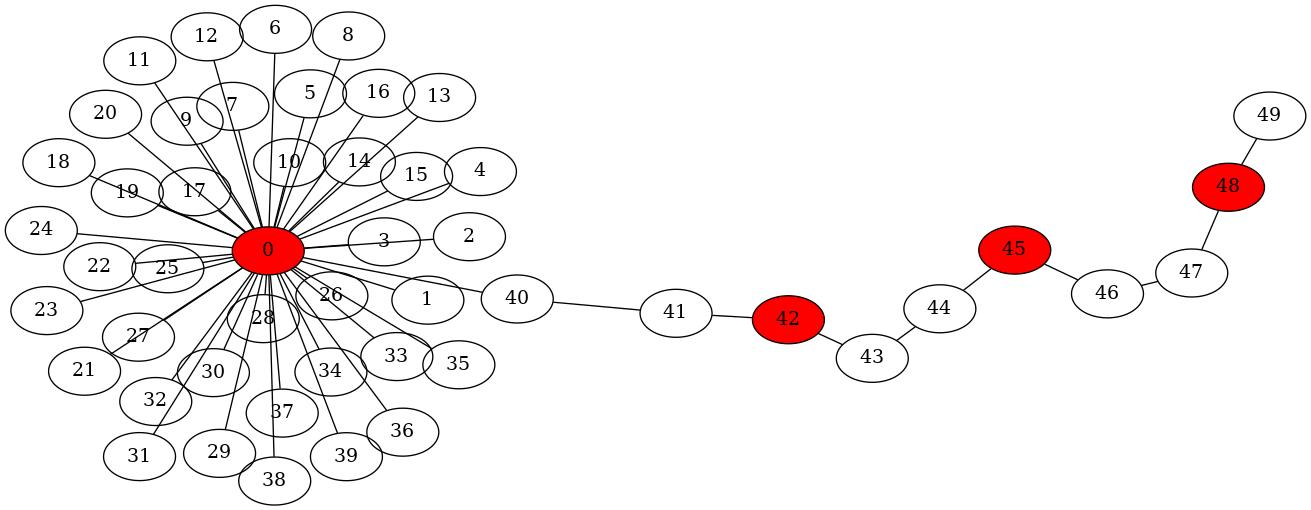
\includegraphics[scale=0.25]{star-chain}
\caption{Star-chain graph, with optimal dominating set in red}
\end{figure}
Nodes 41-49 are \alert{missing on a lot of information} !
\end{frame}

\begin{frame}{Follow Best Informed (FBI) policy}
\begin{itemize}
\item FYL policy is myopic 
\item In addition to their previous action, nodes can output the number of samples (information) they used to compute it
\item Nodes can \alert{follow their best informed neighbor and use UCB-policy if they are better informed}
\item Actually, the structure of a graph fully determines the behavior of the nodes (but not their precise actions obviously)
\end{itemize}
\end{frame}

\begin{frame}{Example of the usefulness of the FBI policy}
\begin{figure}
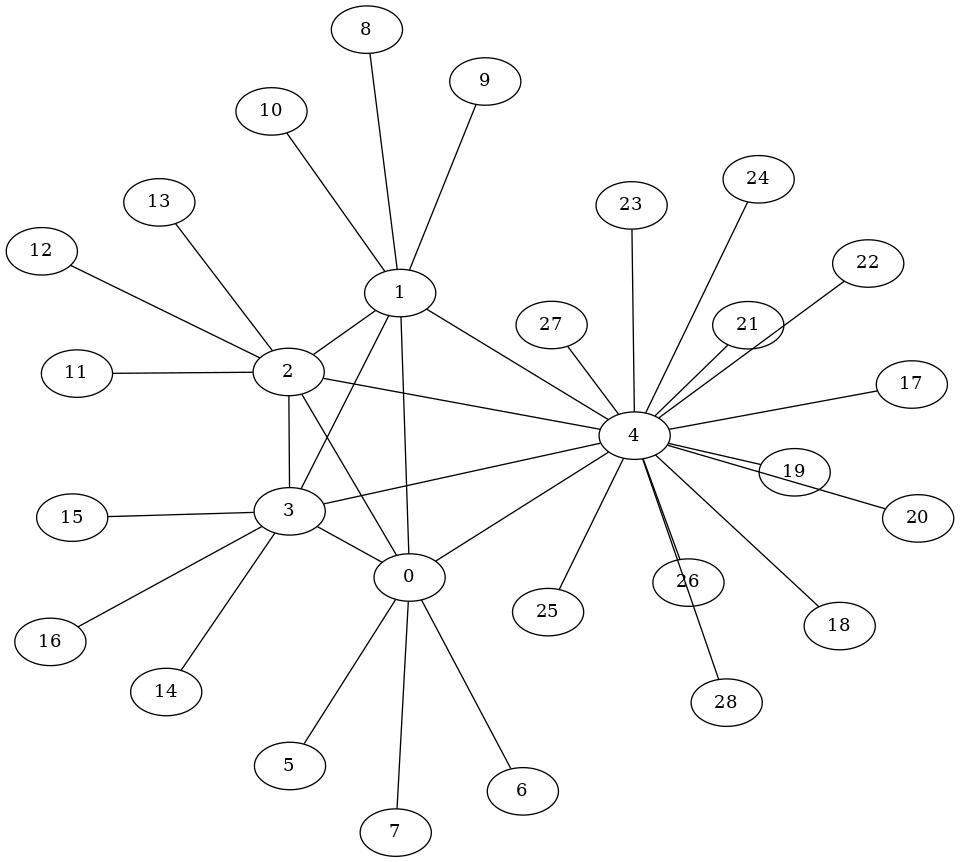
\includegraphics[scale=0.18]{fcstars}
\caption{\centering Fully connected stars graph}
After first iteration, node 4 has the most information. It can pass it to nodes 0-3, who will then pass it to their children. 
\end{figure}
\end{frame}

\begin{frame}{Results for a fully connected stars graph}
\begin{figure}[H]
  \centering
  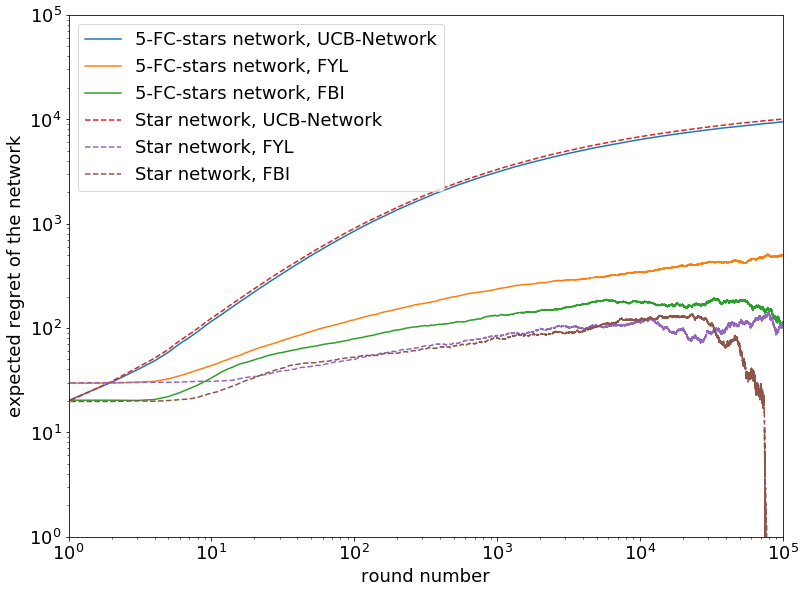
\includegraphics[width=0.49\linewidth]{fig4_1.png}
  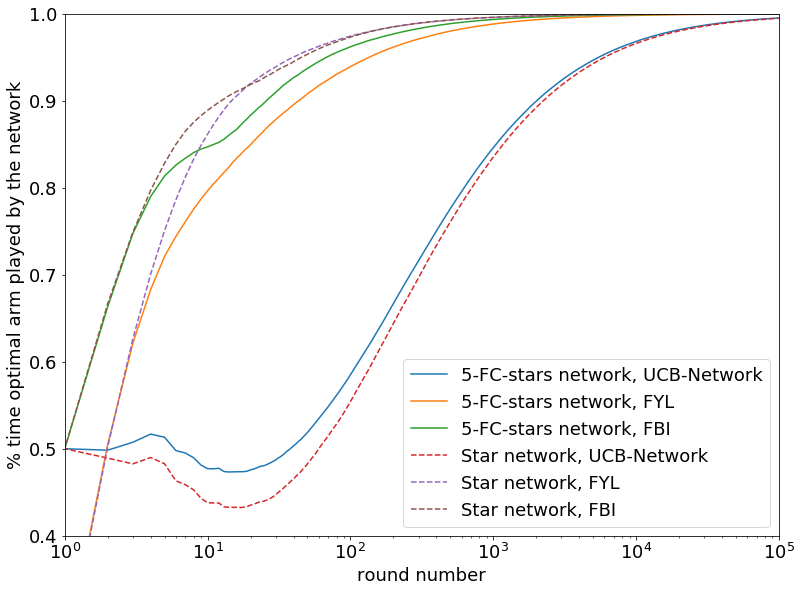
\includegraphics[width=0.49\linewidth]{fig4_2.png}
  \caption{\centering Performance comparison of UCB-Network, FYL, and FBI policies on a 100-nodes star network and on the 100-nodes 5-FC-stars network: 2 arms, Bernoulli rewards with means $0.5$ and $0.7$ (1000 sample paths).}
\end{figure}
\end{frame}

\begin{frame}{Results star-chain graph}
\begin{figure}[H]
  \centering
  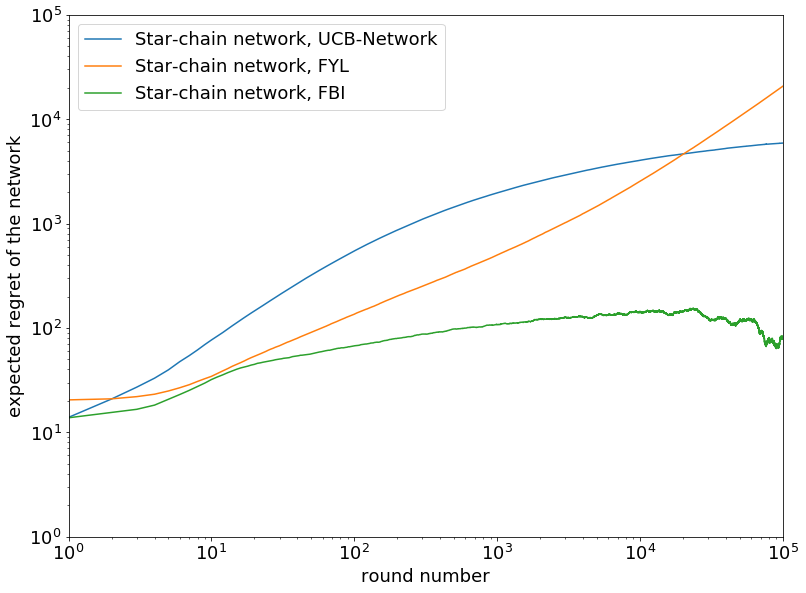
\includegraphics[width=0.49\linewidth]{fig5_1.png}
  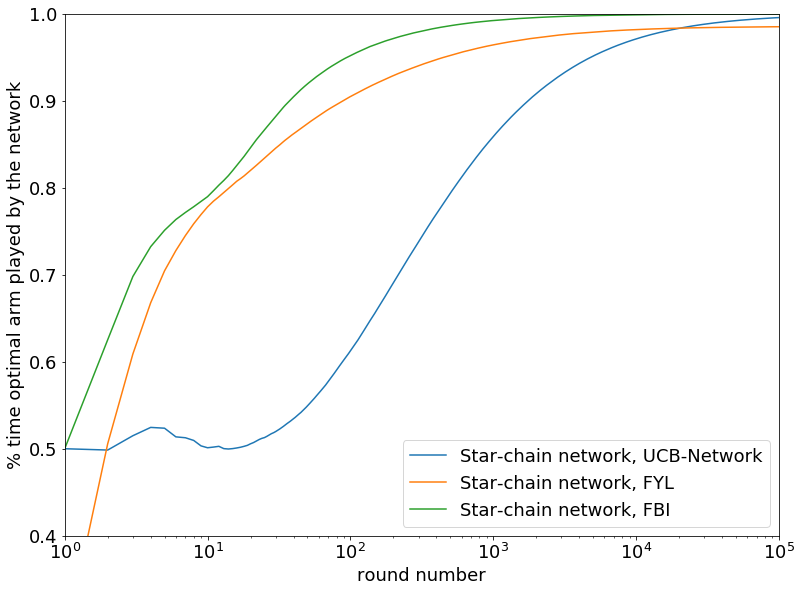
\includegraphics[width=0.49\linewidth]{fig5_2.png}
  \caption{\centering Performance comparison of FYL and FBI policies on the pathological graph structure (star graph with 70 nodes, among which a 20-nodes long chain): 2 arms, Bernoulli rewards with means $0.5$ and $0.7$ (1000 sample paths).}
\end{figure}
\end{frame}

\begin{frame}{A deeper look at the FBI policy}
\begin{itemize}
\item \textbf{Downside} : If one node has more information than the rest, every node it going to follow it (at a delayed rate) $\Rightarrow$ \alert{Strong correlation in the nodes actions} \\ ~ \\


\item \textbf{Further improvements} : When a node has multiple neighbors informed about in the same way, it may be smart to randomly follow one with a \alert{probability depending on its amount of information}. But then the behavior of the nodes is not determined by the structure of the graph... 
\end{itemize}
\end{frame}

\begin{frame}{Conclusion}
\begin{itemize}
\item RL framework very useful to study to study a bandit problem on a graph...
\item ... But the naive solution is not very efficient!
\item For simple policies, interesting bounds can be computed
\item More general types of graphs provide hints to build more robust strategies
\end{itemize}

\end{frame}

\begin{frame}{Thank you}
\centering \Huge Any Questions ?
\end{frame}

\begin{frame}
\AtNextBibliography{\tiny}
\printbibliography
\end{frame}


\end{document}
